%!TEX root = ../index.tex

\section{Deprecated Libraries}
\label{sec:deprecated_libraries}
Der Punkt \ref{f:deprecatedlibraries} ist theoretisch automatisch testbar. Man könnte dem Precommit Hook entsprechende Logik einbauen. In der Praxis ist es jedoch nicht sinnvoll eine Webseite als Fehlerhaft zu markieren nur weil es teile einer Library braucht welche in der nächsten Version nicht mehr vorhanden sind. Darum wurde zusammen mit der Informatikleitung entschieden, dass dieses Fehlerszenario beim Abschluss eines Projektes von Hand geprüft werden soll. Der Go-Live Checkliste wurde ein Punkt hinzugefügt um diesen Punkt abzudecken.

\section{Wiederkehrende manuelle Tests}
\label{sec:wiederkehrende_manuelle_tests}
Zusätzlich zu der bestehenden Go-Live Checkliste wurde eine Checkliste erstellt, welche bei Webprojekten nach dem Go-Live regelmässig durchgegangen wird. Diese Checkliste ist in Tabelle~\ref{tab:recuring_checklist} ersichtlich.

\makeatletter
\newcounter{tnumber} \setcounter{tnumber}{0}
\renewcommand\thetnumber{T\arabic{tnumber}}
\newcommand{\newtnumber}[3]%
{%
\midrule%
\refstepcounter{tnumber}%
\expandafter\xdef\csname t#2\endcsname {#1}%
\thetnumber\label{t:#2} & #1 & #3 \\
}
\makeatother

\begin{table}[ht]
  \centering
  \begin{tabular}{l>{\raggedright} p{10cm} p{2cm}}
    \toprule \textbf{Nr.} & \textbf{Test} & \textbf{Abgedeckte Fehlerszenarios} \\
    \newtnumber{Funktioniert die Webseite erwartungsgemäss? Ist offensichtliches Fehlverhalten vorhanden?}{missverhalten}{\ref{f:missverhalten}}
    \newtnumber{Sind die verwendeten Versionen von Django, feincms etc. noch aktuell?}{abhaengigkeitenmitsicherheitsluecken}{\ref{f:abhaengigkeitenmitsicherheitsluecken}}
    \newtnumber{Funktioniert die Seite in den aktuellen Versionen von Safari, Firefox, Chrome und IE?}{browserspezifischeprobleme}{\ref{f:browserspezifischeprobleme}}
    \newtnumber{Sind auf der Startseite und den Landingpages offensichtliche Rechtschreibefehler?}{rechtschreibefehler}{\ref{f:rechtschreibefehler}}
    \newtnumber{Sind die verwendeten Bilder richtig aufbereitet?}{falschaufbereitetebilder}{\ref{f:falschaufbereitetebilder}}
    \newtnumber{Wurde das Design offensichtlich verletzt?}{designverletzt}{\ref{f:designverletzt}}
    \bottomrule
  \end{tabular}
  \caption{Checkliste für wiederkehrende Überprüfungen}
  \label{tab:recuring_checklist}
\end{table}

\section{Continuous Integration}
\label{sec:continuous_integration_proof_of_concept}
Da Travis für Unternehmen zur Zeit noch nicht frei verfügbar ist, wurde Travis angeschrieben und unsere Situation geschildert. Darauf erhielt allink die benötigte Einladung um Travis zu benutzen.
Um Travis in den bestehenden Projekt Workflow zu integrieren, wurde im der Basiscodebase welche für jedes Django Softwareprojekt verwendet wurde ein .travis.yml erstellt, welches die genaue Testkonfiguration und den Ablauf beinhaltet.

\section{Monitoring}
\label{sec:monitoring_proof_of_concept}
Um alles Webprojekte automatisiert zu überprüfen wurden zwei neue Systeme eingeführt und ein bereits bestehendes System erweitert.

\subsection{Status Cake}
\label{sub:status_cake}
Als erstes neues System wurde Status Cake für alle Webprojekte eingeführt. Damit wird im Minutentakt überprüft, ob die Seiten noch erreichbar sind und ob mit den SSL Zertifikaten alles in Ordnung ist. Zudem werden einmal täglich alle Webseiten nach toten Links durchsucht.

Damit die Tests in Status Cake nicht von Hand nachgetragen werden müssen, wurde der allink.planer so erweitert, dass er Webprojekte automatisch beim Erfassen direkt zu Status Cake hinzufügt.

\begin{figure}[ht]
\centering
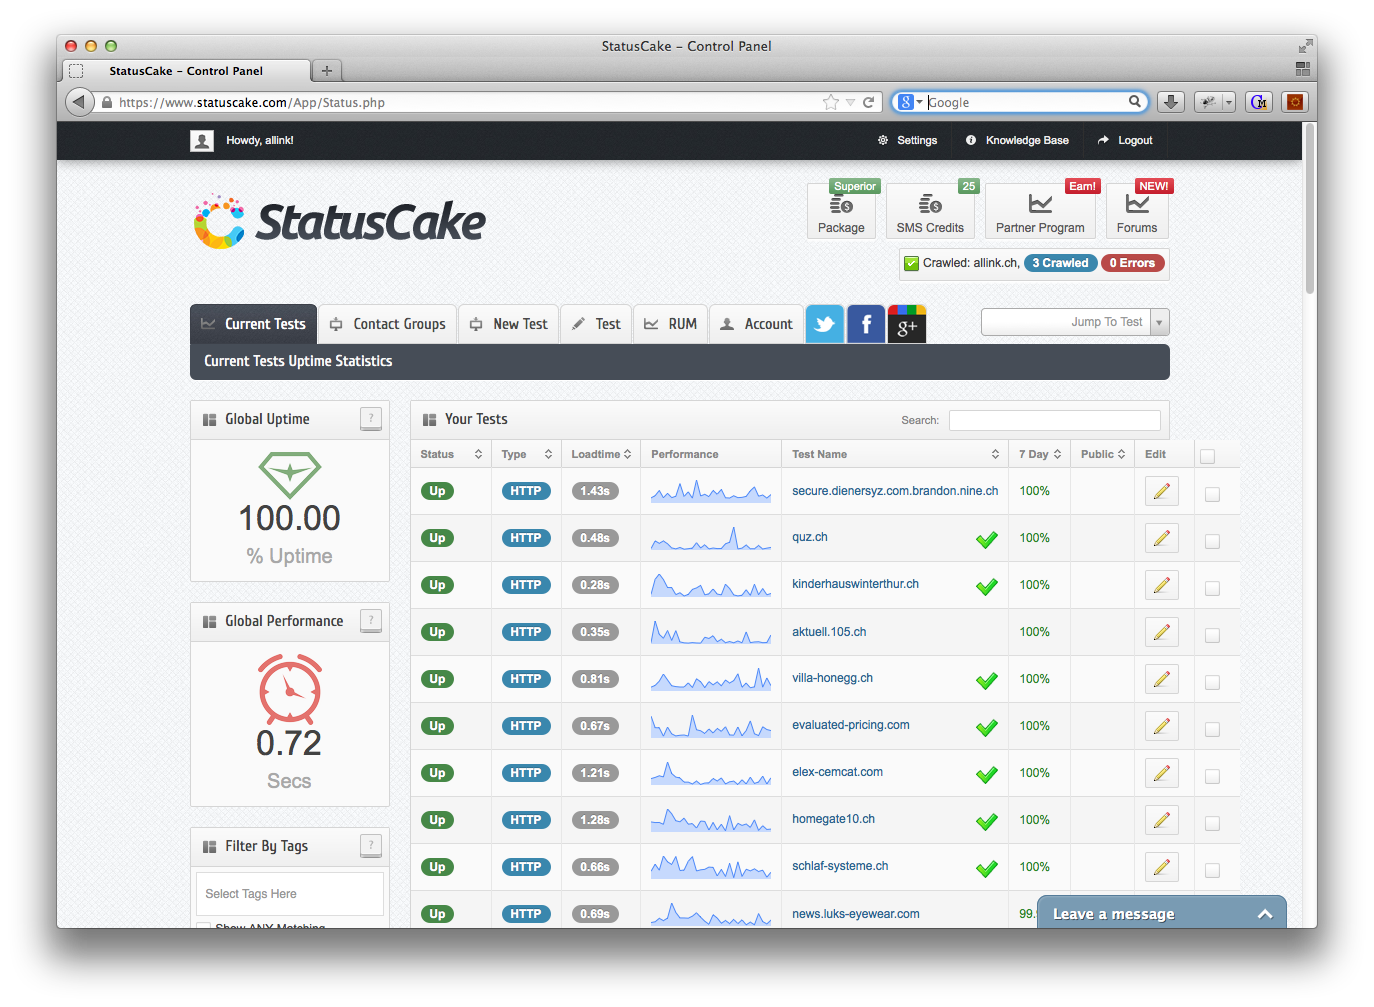
\includegraphics[width=1\textwidth]{images/status_cake.png}
\caption{Status Cake Übersicht}
\label{fig:status_cake}
\end{figure}


\subsection{New Relic}
\label{sub:new_relic}
Weiterhin wurde für einige Webprojekte New Relic eingeführt. Ein bestehendes Projekt mit New Relic auszurüsten ist einiges Aufwendiger, als es mit Status Cake auszurüsten. Für die Integration von New Relic müssen Änderungen am Programmcode vorgenommen werden. Dies ist bei neuen Projekten kein Problem, da für neue Projekte ein Template verwendet wird.

Das Preismodel von New Relic berechnet die Kosten anhand der Anzahl Server welche verwendet werden. Da in der allink demnächst ein grosser Teil der Produktiven Systeme ersetzt werden und danach auch weniger Server eingesetzt werden, wird mit dem Einsatz von New Relic für alle Projekte gewartet, bis diese Umstellung erfolgt ist. Bis dahin werden nur zwei Projekte mit New Relic ausgestattet.

New Relic bietet unter anderem eine Mobile Applikation welche die wichtigsten Daten einer Webseite anzeigen kann. Zudem gibt es für jedes Projekt ein Dashboard wie in Abbildung~\ref{fig:new_relic_dashboard} gezeigt wird, auf welchem man Probleme jeder Art schnell erkennen kann.

\begin{figure}[ht]
\centering
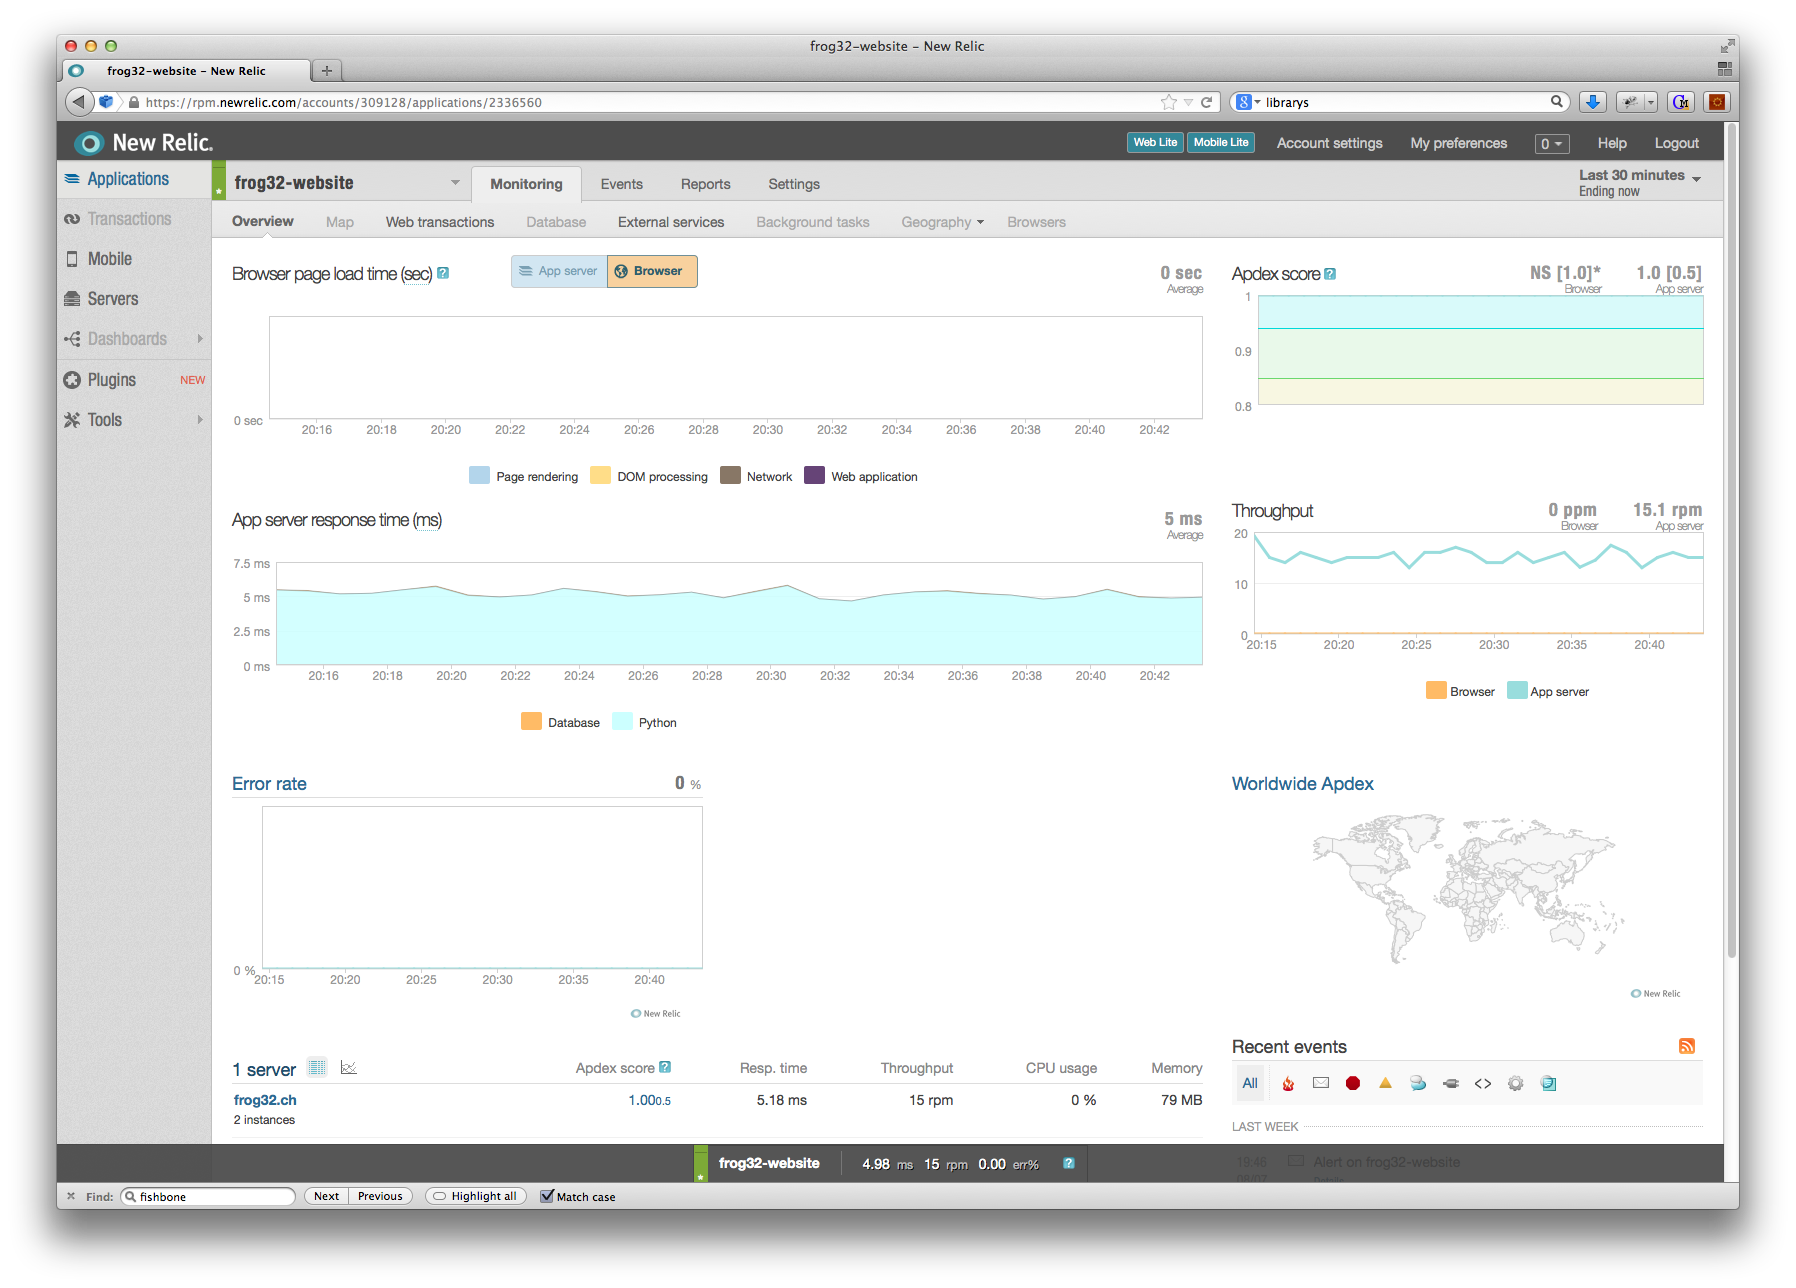
\includegraphics[width=1\textwidth]{images/new_relic.png}
\caption{New Relic Dashboard}
\label{fig:new_relic_dashboard}
\end{figure}


\subsection{allink.planer}
\label{sub:proof_allink_planer}
Der allink.planer wurde wo erweitert, dass er die Fehlerszenarios \ref{f:sslnichterzwungen}, \ref{f:spfeintragfehlerhaft} und \ref{f:debugmodus} abdecken kann. Dies sind alles Fehlerszenarios welche ohne Probleme von ausserhalb eines Webprojektes überprüfbar sind. Weiterhin wurde der allink.planer so erweitert, dass er fähig ist die Versionen von verwendeten Python Paketen jedes Projektes auszulesen. Damit lässt sich im Falle, dass eine Sicherheitslücke bekannt wird schnell feststellen in welchen Projekten die betroffenen Softwareversionen eingesetzt wurden. Damit wird das manuelle Überprüfen von Fehlerszenario \ref{f:abhaengigkeitenmitsicherheitsluecken} massiv vereinfacht.

\section{Auswirkungen}
\label{sec:auswirkungen}
Mit all den neuen Tools wurde auch die Menge an E-Mails welche jeder Entwickler täglich erhält stetig grösser. So versendet zum Beispiel Status Cake jedes mal ein E-Mail, wenn eine zu überwachende Seite nicht mehr erreichbar ist. Dies führte dazu, dass die meisten Entwickler diese E-Mails mittels Regeln direkt in eigene Ordner verschieben lassen. So fällt es nicht mehr direkt auf, wenn eine Webseite nicht mehr erreichbar ist, da das E-Mail welches darauf hinweisen soll, automatisch aus dem Posteingang entfernt wird und in einen eigenen Ordner bewegt wird welche für solche Benachrichtigungen vorgesehen ist. Dadurch bleibt übrigen E-Mails im Posteingang mehr Aufmerksamkeit, jedoch kann es vorkommen, dass ein schwerwiegender Fehler über einen Tag nicht bemerkt wird.

E-Mails welche von Sentry versendet werden teilweise ignoriert, da die Fehler auch in Sentry selber noch angezeigt werden. Leider haben sich zuwenig Entwickler regelmässig die Fehlerliste in Sentry oder die Status Seite von Travis angesehen. Dies führte dazu, dass die gewünschte Wirkung nicht ganz erzielt wurde.

\subsection{Status Monitor}
\label{sub:status_monitor}
Um sicherzustellen, dass Fehler auch wahrgenommen werden, wurde als Zusatz zu den bereits eingeführten Systemen ein Status Monitor eingeführt. Ein Bildschirm welcher vom Arbeitsplatz sämtlicher Entwickler sichtbar ist wurde mit einem am VESA Mount des Displays befestigten Computer ausgestattet. Dabei wurde darauf geachtet, dass der Computer genügend Leistung hat um in einem Webbrowser eine Javascript Applikation ohne Probleme zu betreiben und dass der Stromverbrauch des Computers deutlich unter dem Nivea eines Arbeitsplatzcomputers ist, da dieser Computer ununterbrochen laufen wird.

\subsubsection{Software}
\label{ssub:software}
Das Backend der Software welche die Daten aus verschiedenen Quellen aggregiert wurde mit dem Twisted\footnote{\url{http://twistedmatrix.com/}} Framework in der Programmiersprache Python erstellt. Das Interface welches im Webbrowser läuft wurde als Backbone\footnote{\url{http://backbonejs.org/}} Applikation realisiert um auch Clientseitig eine Templateengine zu haben.

Das Frontend kommuniziert mit dem Backend über einen Websocket. Damit lassen sich Daten asynchron zwischen Frontend und Backend austauschen. Die ganze Software wurde modular aufgebaut damit sich in Zukunft weitere Syteme daran anbinden lassen.

\begin{figure}[ht]
\centering
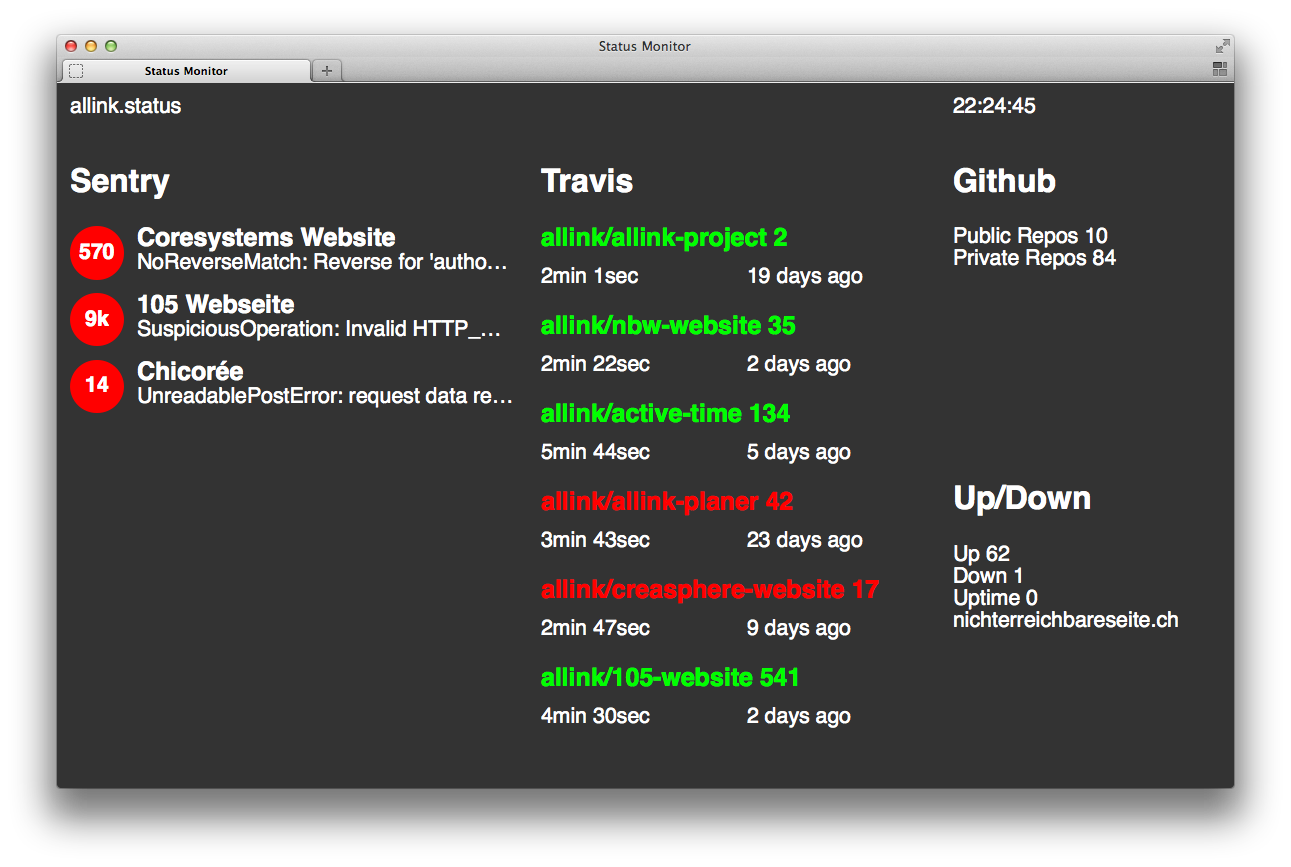
\includegraphics[width=1\textwidth]{images/status_monitor.png}
\caption{Status Monitor}
\label{fig:status_monitor}
\end{figure}
